\chapter{Introducció als grafs}

Molts problemes de programació es poden resoldre modelant el problema
com un problema de grafs i fent servir l'algorisme de grafs
adequat. Un exemple típic de grafs és la xarxa de carreteres i ciutats
d'un país. De vegades, però, el graf està amagat dins del problema i
pot ser difícil detectar-lo.

Aquesta part del llibre tracta els algorismes de grafs, especialment
centrant-se en temes importants en la programació competitiva. En
aquest capítol, repassem conceptes relacionats amb els grafs i
estudiem diferents maneres de representar els grafs en algorismes.

\section{Vocabulari de grafs}

\index{graf} \index{node} \index{aresta}

Un \key{graf} consta de \key{nodes} i \key{arestes}. En aquest llibre,
la variable $n$ indica el nombre de nodes en un graf i la variable $m$
indica el nombre d'arestes. Els nodes es numeren fent servir nombres
$1,2,\ldots,n$.

Per exemple, el graf següent consta de 5 nodes i 7 arestes:


\begin{center}
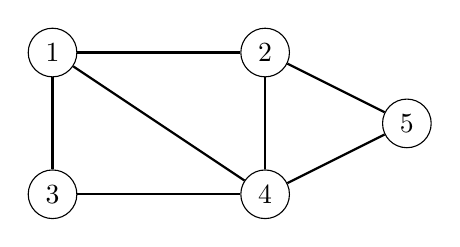
\begin{tikzpicture}[scale=0.9]
\node[draw, circle] (1) at (1,3) {$1$};
\node[draw, circle] (2) at (4,3) {$2$};
\node[draw, circle] (3) at (1,1) {$3$};
\node[draw, circle] (4) at (4,1) {$4$};
\node[draw, circle] (5) at (6,2) {$5$};

\path[draw,thick,-] (1) -- (2);
\path[draw,thick,-] (1) -- (3);
\path[draw,thick,-] (1) -- (4);
\path[draw,thick,-] (3) -- (4);
\path[draw,thick,-] (2) -- (4);
\path[draw,thick,-] (2) -- (5);
\path[draw,thick,-] (4) -- (5);
\end{tikzpicture}
\end{center}


\index{camí}

Un \key{camí} condueix des del node $a$ al node $b$ a través de les
arestes del graf. La \key{longitud} d'un camí és el nombre d'arestes
que té.  Per exemple, el graf anterior conté un camí $1 \rightarrow 3
\rightarrow 4 \rightarrow 5$ de longitud 3 des del node 1 fins al node
5:


\begin{center}
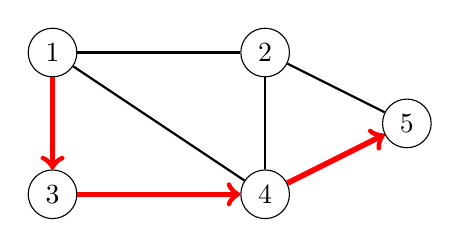
\begin{tikzpicture}[scale=0.9]
\node[draw, circle] (1) at (1,3) {$1$};
\node[draw, circle] (2) at (4,3) {$2$};
\node[draw, circle] (3) at (1,1) {$3$};
\node[draw, circle] (4) at (4,1) {$4$};
\node[draw, circle] (5) at (6,2) {$5$};

\path[draw,thick,-] (1) -- (2);
\path[draw,thick,-] (1) -- (3);
\path[draw,thick,-] (1) -- (4);
\path[draw,thick,-] (3) -- (4);
\path[draw,thick,-] (2) -- (4);
\path[draw,thick,-] (2) -- (5);
\path[draw,thick,-] (4) -- (5);

\path[draw=red,thick,->,line width=2pt] (1) -- (3);
\path[draw=red,thick,->,line width=2pt] (3) -- (4);
\path[draw=red,thick,->,line width=2pt] (4) -- (5);
\end{tikzpicture}
\end{center}


\index{cicle}

Un camí és un \key{cicle} si el primer i l'últim node són el
mateix. Per exemple, el graf anterior conté un cicle $1 \rightarrow 3
\rightarrow 4 \rightarrow 1$. Un camí és \key{simple} si cada node
apareix com a màxim una vegada al camí.



% % \begin{itemize} % \item $1 \rightarrow 2 \rightarrow 5$ (longitud 2) % \item $1 \rightarrow 4 \rightarrow 5$ (longitud 2) % \item $1 \rightarrow 2 \rightarrow 4 \rightarrow 5 $ (longitud 3) % \item $1 \rightarrow 3 \rightarrow 4 \rightarrow 5$ (longitud 3) % \item $1 \rightarrow 4 \rightarrow 2 \rightarrow 5$ (longitud 3) % \item $1 \rightarrow 3 \rightarrow 4 \rightarrow 2 \rightarrow 5$ (longitud 4) % \end{itemize}

\subsubsection{Connectivitat}

\index{graf connex}

Un graf és \key{connex} si hi ha un camí entre dos nodes
qualsevol. Per exemple, el graf següent és connex:
\begin{center}
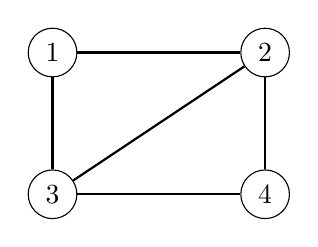
\begin{tikzpicture}[scale=0.9]
\node[draw, circle] (1) at (1,3) {$1$};
\node[draw, circle] (2) at (4,3) {$2$};
\node[draw, circle] (3) at (1,1) {$3$};
\node[draw, circle] (4) at (4,1) {$4$};
\path[draw,thick,-] (1) -- (2);
\path[draw,thick,-] (1) -- (3);
\path[draw,thick,-] (2) -- (3);
\path[draw,thick,-] (3) -- (4);
\path[draw,thick,-] (2) -- (4);
\end{tikzpicture}
\end{center}


El graf següent no és connex, perquè no és possible anar del node 4
a cap altre node:
\begin{center}
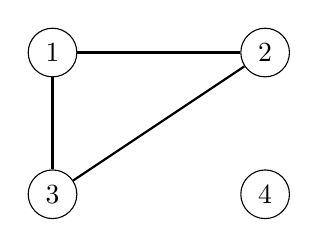
\begin{tikzpicture}[scale=0.9]
\node[draw, circle] (1) at (1,3) {$1$};
\node[draw, circle] (2) at (4,3) {$2$};
\node[draw, circle] (3) at (1,1) {$3$};
\node[draw, circle] (4) at (4,1) {$4$};
\path[draw,thick,-] (1) -- (2);
\path[draw,thick,-] (1) -- (3);
\path[draw,thick,-] (2) -- (3);
\end{tikzpicture}
\end{center}


\index{component}

Les parts connexes d'un graf s'anomenen \key{components connexes}. Per
exemple, el graf següent conté tres components connexes: $\{1,\,2,\,3\}$,
$\{4,\,5,\,6,\,7\}$ i $\{8 \}$.
\begin{center}
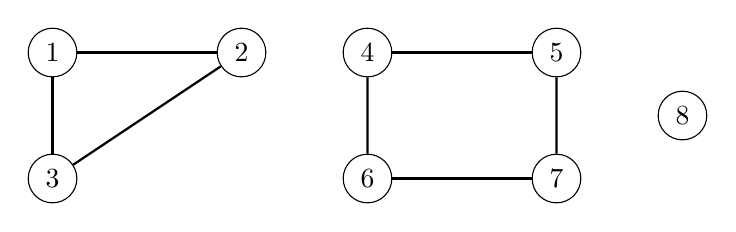
\begin{tikzpicture}[scale=0.8]
\node[draw, circle] (1) at (1,3) {$1$};
\node[draw, circle] (2) at (4,3) {$2$};
\node[draw, circle] (3) at (1,1) {$3$};

\node[draw, circle] (6) at (6,1) {$6$};
\node[draw, circle] (7) at (9,1) {$7$};
\node[draw, circle] (4) at (6,3) {$4$};
\node[draw, circle] (5) at (9,3) {$5$};

\node[draw, circle] (8) at (11,2) {$8$};

\path[draw,thick,-] (1) -- (2);
\path[draw,thick,-] (2) -- (3);
\path[draw,thick,-] (1) -- (3);
\path[draw,thick,-] (4) -- (5);
\path[draw,thick,-] (5) -- (7);
\path[draw,thick,-] (6) -- (7);
\path[draw,thick,-] (6) -- (4);
\end{tikzpicture}
\end{center}


\index{arbre}

Un \key{arbre} és un graf connex que consta de $n$ nodes i $n-1$
arestes. Entre dos nodes quaslevol de l'arbre hi ha un camí únic. Per
exemple, el graf següent és un arbre:


\begin{center}
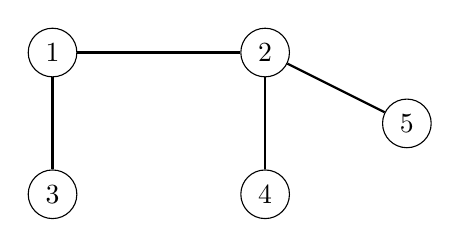
\begin{tikzpicture}[scale=0.9]
\node[draw, circle] (1) at (1,3) {$1$};
\node[draw, circle] (2) at (4,3) {$2$};
\node[draw, circle] (3) at (1,1) {$3$};
\node[draw, circle] (4) at (4,1) {$4$};
\node[draw, circle] (5) at (6,2) {$5$};

\path[draw,thick,-] (1) -- (2);
\path[draw,thick,-] (1) -- (3);
%\path[draw,thick,-] (1) -- (4);
\path[draw,thick,-] (2) -- (5);
\path[draw,thick,-] (2) -- (4);
%\path[draw,thick,-] (4) -- (5);
\end{tikzpicture}
\end{center}


\subsubsection{Arestes dirigides}

\index{graf dirigit}

Un graf és \key{dirigit} si les arestes només es poden recórrer en una
direcció. Per exemple, el graf següent és un graf dirigit:
\begin{center}
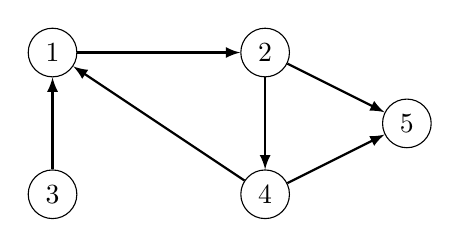
\begin{tikzpicture}[scale=0.9]
\node[draw, circle] (1) at (1,3) {$1$};
\node[draw, circle] (2) at (4,3) {$2$};
\node[draw, circle] (3) at (1,1) {$3$};
\node[draw, circle] (4) at (4,1) {$4$};
\node[draw, circle] (5) at (6,2) {$5$};
\path[draw,thick,->,>=latex] (1) -- (2);
\path[draw,thick,->,>=latex] (2) -- (4);
\path[draw,thick,->,>=latex] (2) -- (5);
\path[draw,thick,->,>=latex] (4) -- (5);
\path[draw,thick,->,>=latex] (4) -- (1);
\path[draw,thick,->,>=latex] (3) -- (1);
\end{tikzpicture}
\end{center}


El graf anterior conté un camí $3 \rightarrow 1 \rightarrow 2
\rightarrow 5$ des del node $3$ fins al node $5$, però no hi ha cap
camí des del node $5$ fins al node $3$.

\subsubsection{Arestes amb pesos}

\index{graf amb pesos}

Un graf té \key{pesos} si a cada aresta se li assigna un
\key{pes}. Els pesos s'interpreten sovint com a longituds de l'aresta. Per
exemple, el graf següent és un graf amb pesos:
\begin{center}
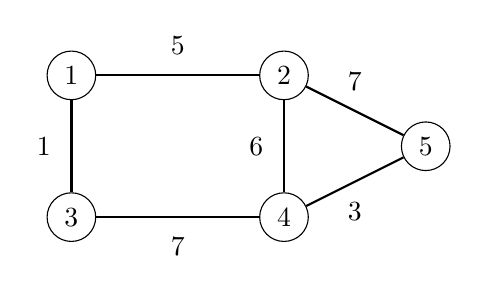
\begin{tikzpicture}[scale=0.9]
\node[draw, circle] (1) at (1,3) {$1$};
\node[draw, circle] (2) at (4,3) {$2$};
\node[draw, circle] (3) at (1,1) {$3$};
\node[draw, circle] (4) at (4,1) {$4$};
\node[draw, circle] (5) at (6,2) {$5$};
\path[draw,thick,-] (1) -- node[font=\small,label=above:5] {} (2);
\path[draw,thick,-] (1) -- node[font=\small,label=left:1] {} (3);
\path[draw,thick,-] (3) -- node[font=\small,label=below:7] {} (4);
\path[draw,thick,-] (2) -- node[font=\small,label=left:6] {} (4);
\path[draw,thick,-] (2) -- node[font=\small,label=above:7] {} (5);
\path[draw,thick,-] (4) -- node[font=\small,label=below:3] {} (5);
\end{tikzpicture}
\end{center}


La longitud d'un camí d'un graf amb pesos és la suma dels pesos de les
arestes del camí. Per exemple, al graf anterior, la longitud del camí
$1 \rightarrow 2 \rightarrow 5$ és $12$ i la longitud del camí $1
\rightarrow 3 \rightarrow 4 \rightarrow 5$ és $11$. Aquest darrer camí
és el camí \key{més curt} des del node $1$ fins al node $5$.

\subsubsection{Veïns i graus}

\index{veí} \index{grau}

Dos nodes són \key{veins} o \key{adjacents} si hi ha una aresta entre
ells. El \key{grau} d'un node és el nombre d'arestes incidents al
node, que coincideix amb el nombre de nodes veins si el graf és
simple. Per exemple, al graf següent, els veïns del node 2 són 1, 4 i
5, de manera que el seu grau és 3.


\begin{center}
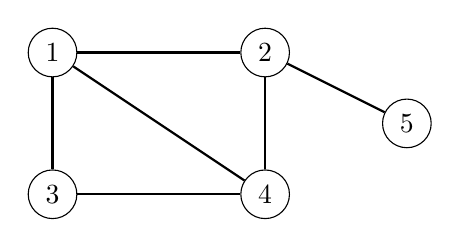
\begin{tikzpicture}[scale=0.9]
\node[draw, circle] (1) at (1,3) {$1$};
\node[draw, circle] (2) at (4,3) {$2$};
\node[draw, circle] (3) at (1,1) {$3$};
\node[draw, circle] (4) at (4,1) {$4$};
\node[draw, circle] (5) at (6,2) {$5$};

\path[draw,thick,-] (1) -- (2);
\path[draw,thick,-] (1) -- (3);
\path[draw,thick,-] (1) -- (4);
\path[draw,thick,-] (3) -- (4);
\path[draw,thick,-] (2) -- (4);
\path[draw,thick,-] (2) -- (5);
%\path[draw,thick,-] (4) -- (5);
\end{tikzpicture}
\end{center}


La suma de graus d'un graf és sempre $2m$, on $m$ és el nombre
d'arestes, perquè cada aresta té dos extrems, i per tant incrementa el
grau de dos nodes en una unitat. Per aquest motiu, la suma dels graus
sempre és un nombre parell.

\index{graf normal} \index{graf complet}

Un graf és \key{regular} si el grau de cada node és una constant
$d$. Un graf és \key{complet} si el graf conté una aresta per cada parell
de nodes i, per tant, cada node té grau $n-1$.

\index{graus} \index{graus externs}

En un graf dirigit, el \key{grau d'entrada} d'un node és el nombre d'arestes
que apunten al node, i el \key{grau de sortida} d'un node és el nombre
d'arestes que surten del node. Per exemple, al graf següent, el grau
d'entrada del node 2 és 2 i el grau de sortida del node 2 és 1.


\begin{center}
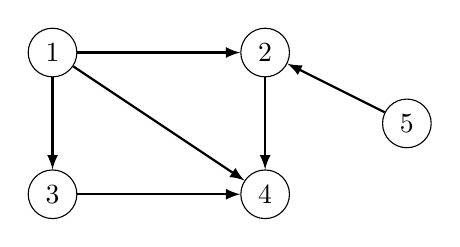
\begin{tikzpicture}[scale=0.9]
\node[draw, circle] (1) at (1,3) {$1$};
\node[draw, circle] (2) at (4,3) {$2$};
\node[draw, circle] (3) at (1,1) {$3$};
\node[draw, circle] (4) at (4,1) {$4$};
\node[draw, circle] (5) at (6,2) {$5$};

\path[draw,thick,->,>=latex] (1) -- (2);
\path[draw,thick,->,>=latex] (1) -- (3);
\path[draw,thick,->,>=latex] (1) -- (4);
\path[draw,thick,->,>=latex] (3) -- (4);
\path[draw,thick,->,>=latex] (2) -- (4);
\path[draw,thick,<-,>=latex] (2) -- (5);
\end{tikzpicture}
\end{center}


\subsubsection{Coloracions}

\index{coloració} \index{graf bipartit}

Una \key{coloració} d'un graf és una assignació de nodes a colors de
manera que no hi hagi dos nodes adjacents amb el mateix color.

Un graf és \key{bipartit} si és possible acolorir-lo amb dos
colors. Es pot demostrar que un graf és bipartit exactament quan no conté cap
cicle amb un nombre senar d'arestes. Per exemple, el graf
[[[11]]]]
és bipartit, perquè es pot acolorir de la següent manera:
\begin{center}
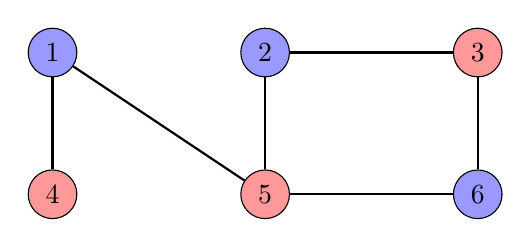
\begin{tikzpicture}[scale=0.9]
\node[draw, circle, fill=blue!40] (1) at (1,3) {$2$};
\node[draw, circle, fill=red!40] (2) at (4,3) {$3$};
\node[draw, circle, fill=red!40] (3) at (1,1) {$5$};
\node[draw, circle, fill=blue!40] (4) at (4,1) {$6$};
\node[draw, circle, fill=red!40] (5) at (-2,1) {$4$};
\node[draw, circle, fill=blue!40] (6) at (-2,3) {$1$};
\path[draw,thick,-] (1) -- (2);
\path[draw,thick,-] (1) -- (3);
\path[draw,thick,-] (3) -- (4);
\path[draw,thick,-] (2) -- (4);
\path[draw,thick,-] (3) -- (6);
\path[draw,thick,-] (5) -- (6);
\end{tikzpicture}
\end{center}
Tanmateix, el graf
\begin{center}
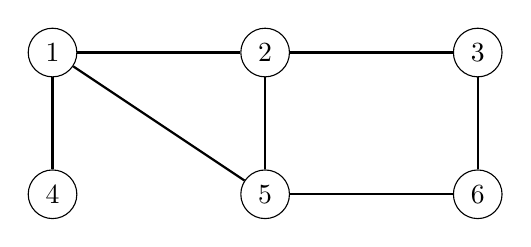
\begin{tikzpicture}[scale=0.9]
\node[draw, circle] (1) at (1,3) {$2$};
\node[draw, circle] (2) at (4,3) {$3$};
\node[draw, circle] (3) at (1,1) {$5$};
\node[draw, circle] (4) at (4,1) {$6$};
\node[draw, circle] (5) at (-2,1) {$4$};
\node[draw, circle] (6) at (-2,3) {$1$};
\path[draw,thick,-] (1) -- (2);
\path[draw,thick,-] (1) -- (3);
\path[draw,thick,-] (3) -- (4);
\path[draw,thick,-] (2) -- (4);
\path[draw,thick,-] (3) -- (6);
\path[draw,thick,-] (5) -- (6);
\path[draw,thick,-] (1) -- (6);
\end{tikzpicture}
\end{center}
no és bipartit, perquè no és possible acolorir el següent cicle de tres
nodes amb dos colors:
\begin{center}
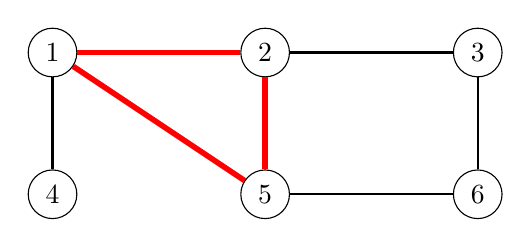
\begin{tikzpicture}[scale=0.9]
\node[draw, circle] (1) at (1,3) {$2$};
\node[draw, circle] (2) at (4,3) {$3$};
\node[draw, circle] (3) at (1,1) {$5$};
\node[draw, circle] (4) at (4,1) {$6$};
\node[draw, circle] (5) at (-2,1) {$4$};
\node[draw, circle] (6) at (-2,3) {$1$};
\path[draw,thick,-] (1) -- (2);
\path[draw,thick,-] (1) -- (3);
\path[draw,thick,-] (3) -- (4);
\path[draw,thick,-] (2) -- (4);
\path[draw,thick,-] (3) -- (6);
\path[draw,thick,-] (5) -- (6);
\path[draw,thick,-] (1) -- (6);

\path[draw=red,thick,-,line width=2pt] (1) -- (3);
\path[draw=red,thick,-,line width=2pt] (3) -- (6);
\path[draw=red,thick,-,line width=2pt] (6) -- (1);
\end{tikzpicture}
\end{center}


\subsubsection{Grafs simples}

\index{graf simple}

Un graf és \key{simple} si cap aresta comença i acaba al mateix node,
i no hi ha múltiples arestes entre dos nodes. Sovint assumim que els
grafs són simples. Per exemple, el graf següent \emph{no} és simple:
\begin{center}
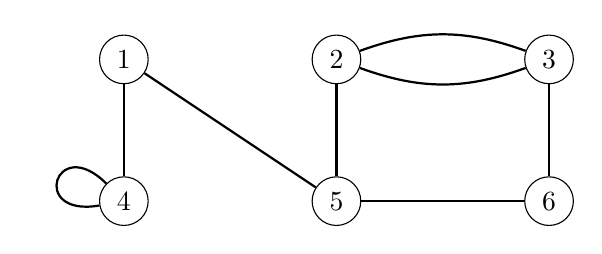
\begin{tikzpicture}[scale=0.9]
\node[draw, circle] (1) at (1,3) {$2$};
\node[draw, circle] (2) at (4,3) {$3$};
\node[draw, circle] (3) at (1,1) {$5$};
\node[draw, circle] (4) at (4,1) {$6$};
\node[draw, circle] (5) at (-2,1) {$4$};
\node[draw, circle] (6) at (-2,3) {$1$};

\path[draw,thick,-] (1) edge [bend right=20] (2);
\path[draw,thick,-] (2) edge [bend right=20] (1);
%\path[draw,thick,-] (1) -- (2);
\path[draw,thick,-] (1) -- (3);
\path[draw,thick,-] (3) -- (4);
\path[draw,thick,-] (2) -- (4);
\path[draw,thick,-] (3) -- (6);
\path[draw,thick,-] (5) -- (6);

\tikzset{every loop/.style={in=135,out=190}}
\path[draw,thick,-] (5) edge [loop left] (5);
\end{tikzpicture}
\end{center}


\section{Representació de grafs}

Hi ha diverses maneres de representar grafs en algorismes. L'elecció
d'una estructura de dades depèn de la mida del graf i de la forma en
què l'algorisme el processa. A continuació mostrarem tres
representacions comunes.

\subsubsection{Llista d'adjacència}

\index{llista d'adjacència}

Per a representar un graf com a llista d'adjacència, assignem a cada
node $x$ del graf una \key{llista d'adjacència} que consta dels nodes
als quals hi ha una aresta des de $x$. Les llistes d'adjacència són la
manera més popular de representar grafs, i la majoria dels algorismes
es poden implementar eficientment amb llistes d'adjacència.

Una manera convenient d'emmagatzemar les llistes d'adjacència és
declarar un \emph{array} de vectors de la manera següent:
\begin{lstlisting}
vector<int> adj[N];
\end{lstlisting}


La constant $N$ s'escull de manera que es pugui emmagatzemar totes
les llistes d'adjacència. Per exemple, el graf


\begin{center}
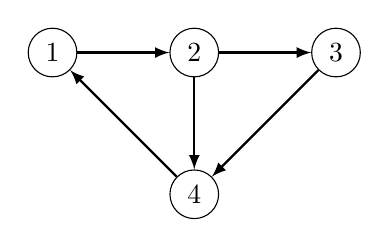
\begin{tikzpicture}[scale=0.9]
\node[draw, circle] (1) at (1,3) {$1$};
\node[draw, circle] (2) at (3,3) {$2$};
\node[draw, circle] (3) at (5,3) {$3$};
\node[draw, circle] (4) at (3,1) {$4$};

\path[draw,thick,->,>=latex] (1) -- (2);
\path[draw,thick,->,>=latex] (2) -- (3);
\path[draw,thick,->,>=latex] (2) -- (4);
\path[draw,thick,->,>=latex] (3) -- (4);
\path[draw,thick,->,>=latex] (4) -- (1);
\end{tikzpicture}
\end{center}
es pot emmagatzemar de la següent manera:
\begin{lstlisting}
adj[1].push_back(2);
adj[2].push_back(3);
adj[2].push_back(4);
adj[3].push_back(4);
adj[4].push_back(1);
\end{lstlisting}


Si el graf no està dirigit, podem fer servir una representació
semblant, però afegim cada aresta en ambdues direccions.

Per a un graf amb pesos, l'estructura es pot ampliar de la següent
manera:


\begin{lstlisting}
vector<pair<int,int>> adj[N];
\end{lstlisting}


En aquest cas, la llista d'adjacència del node $a$ conté el parell
$(b,w)$ sempre quan hi ha una aresta des del node $a$ fins al node $b$
amb pes $w$. Per exemple, el graf


\begin{center}
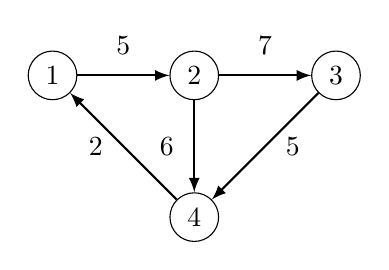
\begin{tikzpicture}[scale=0.9]
\node[draw, circle] (1) at (1,3) {$1$};
\node[draw, circle] (2) at (3,3) {$2$};
\node[draw, circle] (3) at (5,3) {$3$};
\node[draw, circle] (4) at (3,1) {$4$};

\path[draw,thick,->,>=latex] (1) -- node[font=\small,label=above:5] {} (2);
\path[draw,thick,->,>=latex] (2) -- node[font=\small,label=above:7] {} (3);
\path[draw,thick,->,>=latex] (2) -- node[font=\small,label=left:6] {} (4);
\path[draw,thick,->,>=latex] (3) -- node[font=\small,label=right:5] {} (4);
\path[draw,thick,->,>=latex] (4) -- node[font=\small,label=left:2] {} (1);
\end{tikzpicture}
\end{center}
es pot emmagatzemar de la següent manera:
\begin{lstlisting}
adj[1].push_back({2,5});
adj[2].push_back({3,7});
adj[2].push_back({4,6});
adj[3].push_back({4,5});
adj[4].push_back({1,2});
\end{lstlisting}


L'avantatge d'utilitzar llistes d'adjacència és que podem trobar de
manera eficient els nodes als quals ens podem moure des d'un node
determinat a través d'una aresta. Per exemple, el següent bucle passa
per tots els nodes als quals ens podem moure des del node $s$:


\begin{lstlisting}
for (auto u : adj[s]) {
    // fer coses amb el node 'u'
}
\end{lstlisting}


\subsubsection{Matriu d'adjacència}

\index{matriu d'adjacència}
Una \key{matriu d'adjacència} és una matriu bidimensional que indica
quines arestes pertanyen al graf. Amb una matriu d'adjacència podem
comprovar de manera eficient si hi ha una aresta entre dos nodes. La
matriu es pot emmagatzemar com un \emph{array} de vectors
\begin{lstlisting}
int adj[N][N];
\end{lstlisting}
on cada valor $\texttt{adj}[a][b]$ indica si el graf conté una aresta des del node $a$ fins al node $b$. Si l'aresta s'inclou al graf, llavors $\texttt{adj}[a][b]=1$, i en cas contrari $\texttt{adj}[a][b]=0$. Per exemple, el graf
\begin{center}
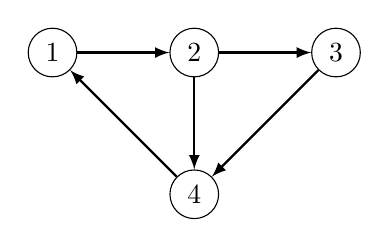
\begin{tikzpicture}[scale=0.9]
\node[draw, circle] (1) at (1,3) {$1$};
\node[draw, circle] (2) at (3,3) {$2$};
\node[draw, circle] (3) at (5,3) {$3$};
\node[draw, circle] (4) at (3,1) {$4$};

\path[draw,thick,->,>=latex] (1) -- (2);
\path[draw,thick,->,>=latex] (2) -- (3);
\path[draw,thick,->,>=latex] (2) -- (4);
\path[draw,thick,->,>=latex] (3) -- (4);
\path[draw,thick,->,>=latex] (4) -- (1);
\end{tikzpicture}
\end{center}
es pot representar de la següent manera:
\begin{center}
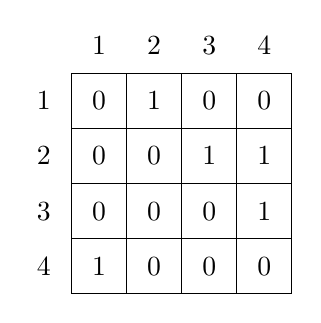
\begin{tikzpicture}[scale=0.7]
\draw (0,0) grid (4,4);
\node at (0.5,0.5) {1};
\node at (1.5,0.5) {0};
\node at (2.5,0.5) {0};
\node at (3.5,0.5) {0};
\node at (0.5,1.5) {0};
\node at (1.5,1.5) {0};
\node at (2.5,1.5) {0};
\node at (3.5,1.5) {1};
\node at (0.5,2.5) {0};
\node at (1.5,2.5) {0};
\node at (2.5,2.5) {1};
\node at (3.5,2.5) {1};
\node at (0.5,3.5) {0};
\node at (1.5,3.5) {1};
\node at (2.5,3.5) {0};
\node at (3.5,3.5) {0};
\node at (-0.5,0.5) {4};
\node at (-0.5,1.5) {3};
\node at (-0.5,2.5) {2};
\node at (-0.5,3.5) {1};
\node at (0.5,4.5) {1};
\node at (1.5,4.5) {2};
\node at (2.5,4.5) {3};
\node at (3.5,4.5) {4};
\end{tikzpicture}
\end{center}


Si el graf té pesos, la representació amb matriu d'adjacència s'extén
de manera que la matriu contingui el pes a l'aresta si l'aresta
existeix. Utilitzant aquesta representació, el graf


\begin{center}
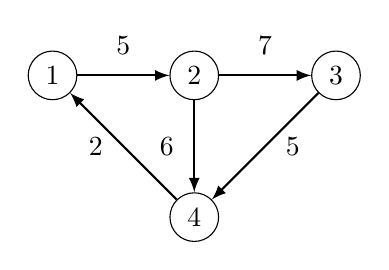
\begin{tikzpicture}[scale=0.9]
\node[draw, circle] (1) at (1,3) {$1$};
\node[draw, circle] (2) at (3,3) {$2$};
\node[draw, circle] (3) at (5,3) {$3$};
\node[draw, circle] (4) at (3,1) {$4$};

\path[draw,thick,->,>=latex] (1) -- node[font=\small,label=above:5] {} (2);
\path[draw,thick,->,>=latex] (2) -- node[font=\small,label=above:7] {} (3);
\path[draw,thick,->,>=latex] (2) -- node[font=\small,label=left:6] {} (4);
\path[draw,thick,->,>=latex] (3) -- node[font=\small,label=right:5] {} (4);
\path[draw,thick,->,>=latex] (4) -- node[font=\small,label=left:2] {} (1);
\end{tikzpicture}
\end{center}

\begin{samepage}
es correspon amb la matriu següent:
\begin{center}
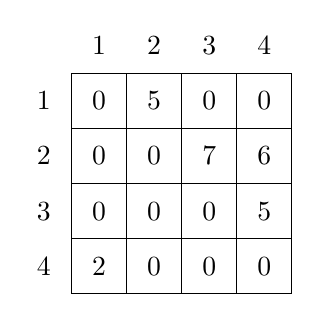
\begin{tikzpicture}[scale=0.7]
\draw (0,0) grid (4,4);
\node at (0.5,0.5) {2};
\node at (1.5,0.5) {0};
\node at (2.5,0.5) {0};
\node at (3.5,0.5) {0};
\node at (0.5,1.5) {0};
\node at (1.5,1.5) {0};
\node at (2.5,1.5) {0};
\node at (3.5,1.5) {5};
\node at (0.5,2.5) {0};
\node at (1.5,2.5) {0};
\node at (2.5,2.5) {7};
\node at (3.5,2.5) {6};
\node at (0.5,3.5) {0};
\node at (1.5,3.5) {5};
\node at (2.5,3.5) {0};
\node at (3.5,3.5) {0};
\node at (-0.5,0.5) {4};
\node at (-0.5,1.5) {3};
\node at (-0.5,2.5) {2};
\node at (-0.5,3.5) {1};
\node at (0.5,4.5) {1};
\node at (1.5,4.5) {2};
\node at (2.5,4.5) {3};
\node at (3.5,4.5) {4};
\end{tikzpicture}
\end{center}
\end{samepage}


L'inconvenient de la representació amb matrius d'adjacència és que la
matriu conté $n^2$ elements, i normalment la majoria d'ells són
zero. Per aquest motiu, la representació no es pot fer servir si el
graf és gran.

\subsubsection{Llista d'arestes}

\index{llista d'aresta}

Una \key{llista d'arestes} conté totes les arestes d'un graf en un
cert ordre. Aquesta és una manera convenient de representar un graf si
l'algorisme processa totes les arestes del graf i no cal trobar les
arestes que comencen en un node determinat.

La llista d'arestes es pot emmagatzemar en un vector
\begin{lstlisting}
vector<pair<int,int>> edges;
\end{lstlisting}
on cada parell $(a,b)$ indica que hi ha una aresta des del node $a$
fins al node $b$. Així, el graf


\begin{center}
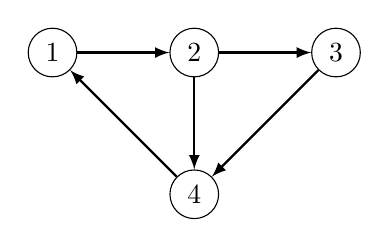
\begin{tikzpicture}[scale=0.9]
\node[draw, circle] (1) at (1,3) {$1$};
\node[draw, circle] (2) at (3,3) {$2$};
\node[draw, circle] (3) at (5,3) {$3$};
\node[draw, circle] (4) at (3,1) {$4$};

\path[draw,thick,->,>=latex] (1) -- (2);
\path[draw,thick,->,>=latex] (2) -- (3);
\path[draw,thick,->,>=latex] (2) -- (4);
\path[draw,thick,->,>=latex] (3) -- (4);
\path[draw,thick,->,>=latex] (4) -- (1);
\end{tikzpicture}
\end{center}
es pot representar de la següent manera:
\begin{lstlisting}
edges.push_back({1,2});
edges.push_back({2,3});
edges.push_back({2,4});
edges.push_back({3,4});
edges.push_back({4,1});
\end{lstlisting}


\noindent Si el graf té pesos, l'estructura es pot ampliar de la següent manera:
\begin{lstlisting}
vector<tuple<int,int,int>> edges;
\end{lstlisting}
Cada element d'aquesta llista té la forma $(a,b,w)$, el que significa que hi ha una aresta des del node $a$ fins al node $b$ amb pes $w$. Per exemple, el graf


\begin{center}
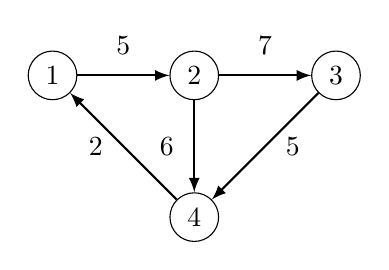
\begin{tikzpicture}[scale=0.9]
\node[draw, circle] (1) at (1,3) {$1$};
\node[draw, circle] (2) at (3,3) {$2$};
\node[draw, circle] (3) at (5,3) {$3$};
\node[draw, circle] (4) at (3,1) {$4$};

\path[draw,thick,->,>=latex] (1) -- node[font=\small,label=above:5] {} (2);
\path[draw,thick,->,>=latex] (2) -- node[font=\small,label=above:7] {} (3);
\path[draw,thick,->,>=latex] (2) -- node[font=\small,label=left:6] {} (4);
\path[draw,thick,->,>=latex] (3) -- node[font=\small,label=right:5] {} (4);
\path[draw,thick,->,>=latex] (4) -- node[font=\small,label=left:2] {} (1);
\end{tikzpicture}
\end{center}

\begin{samepage}
es pot representar com segueix\footnote{En alguns compiladors
antics, és necessari fer servir la funció \texttt{make\_tuple} en lloc de
les claus (per exemple, \texttt{make\_tuple(1,2,5)} en lloc de
\texttt{\{1,2,5\}}).}:  
\begin{lstlisting}
edges.push_back({1,2,5});
edges.push_back({2,3,7});
edges.push_back({2,4,6});
edges.push_back({3,4,5});
edges.push_back({4,1,2});
\end{lstlisting}
\end{samepage}
